\section{Introduction}

Multi-class classification is a generalization of the multi-label classification where one instance can be assigned to multiple classes.
We take this further and work with a multi-output (a specific case of multi-task) mixed multi-label/multi-class classification task.
We focus on one specific classification task though its selection is arbitrary and we believe that the results are highly transferable to other tasks.
The input samples are articles (headlines and bodies) and the outputs are either one of multiple classes (variables \emph{newspaper, newspaper political alignment, newspaper country, year, month}) or a non-empty subset of classes (variables \emph{subject topics, geographic topics}).
We compare various approaches to this complicated task and mainly focus on how having a partial answer to the output, such as answers to one of the outputs, affects the performance and model computation.
Advancements in this task may be of interest in applications where partial information is provided by empirical data collection, by an expert directly or by large scale information retrieval.
In such cases, the extra information is either not available for every sample or non-trivial to obtain.

\paragraph{Contribution.}
This paper aims to answer the following questions through a series of experiments with text classification and leveraging pre-trained language models:
\begin{enumerate}[left=0.4cm,itemsep=0cm]
\item Is joint multi-output learning better than using separate models for individual outputs?
\item Does providing partial answers help in the classification of other outputs?
\item Is it possible to predict when a model will require access to partial answers to make correct classification? 
\item How does the fusion affect the model computation for correct, incorrect classifications and in cases where correct or incorrect help was provided?
\end{enumerate}

% move the fig here to force be on top of the second page
\begin{figure*}[ht]
\centering
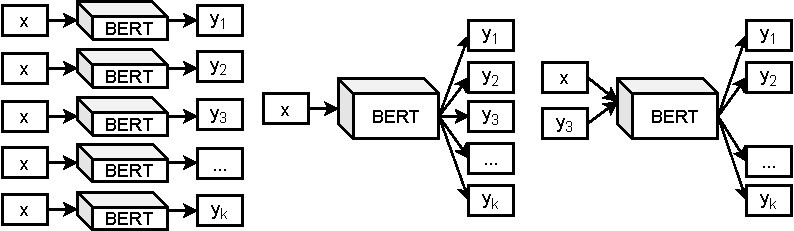
\includegraphics[width=0.85\textwidth]{img/diagram_overview.pdf}
\caption{Different modes of approaching multi-task learning: individual model (left) and joint model (center, right). The joint model is also enhanced with one output variable as input (right).}
\label{fig:diagram_overview}
\end{figure*}

The first and the second point is interesting for determining whether it makes sense to build larger joint versatile models that solve multiple classification problems and whether we should be trying to provide the models with as much extra information as possible.
Intuitively, knowing the \emph{newspaper country} of the article should help in narrowing down the \emph{geographic topics} because of different newspaper foci. 
The third point is motivated by scenarios in which requesting additional knowledge bears costs (e.g. compute time for retrieval or money for annotation).
The last point aims to provide the first step towards a deeper understanding of how priming affects model computation.
Our goal is not to find the best model that solves a particular multi-output classification scenario but to examine the issue of fusion and provision of artefacts.

\paragraph{Content.}
The data, methodology and used models are introduced in \Cref{sec:methods}.
Comparison of using individual models vs. a single joint one, experiments with the fusion of artefacts, predicting the need for them and fusion tracing are presented in \Cref{sec:experiments}.
For completeness, we provide the performance of other baseline models (SVM and LSTM with pre-trained word embeddings) in \Cref{subsubsec:baselines}.
We conclude together with areas for future research in \Cref{sec:conclusion}.
The code for this project is available open-source.\footnote{
\href{https://github.com/zouharvi/partial-answers-artefacts}{github.com/zouharvi/partial-answers-artefacts}
}

\subsection{Related Work} \label{subsec:related}

The task of multi-output learning has been thoroughly surveyed by \newcite{borchani2015survey} and \newcite{multioutput_learning}.
We, therefore, skip the formal mathematical definition of the classification task in favour of these works.
Multi-output and, in general, multi-task learning has seen a wide range of applications in recent years because of the ability to leverage joint hidden representation \cite{yao2020exploiting,proencca2020quadruplet}.
It has also been widely applied to NLP classification tasks using foundation models \cite{jiang2019multi,xin2020early,suhane2021multi}.

Related to our third research question, predicting the need for artefacts, \newcite{he2021efficient} have trained a language model which is able to dynamically retrieve from a knowledge-base (built during training).
Because of the high computation cost of retrieval, they also implemented a meta-model that determines whether the model needs this retrieval (e.g. retrieval not needed for common, easy words but needed for entities).
We follow up on this by trying to predict which artefact specifically to fuse to ensure a better prediction.

We study the task through the lenses of the formalism of artefacts introduced by \newcite{zouhar2021artefact}.
An artefact, in general, is an object which can be fused into the original model to improve its performance.
In the context of question answering it is the retrieved relevant documents but for e.g., fact-aware language modelling \cite{logan2019barack} it may be retrieving facts related to the to-be-predicted entity.
Although its origins are in research on information retrieval and knowledge-intensive tasks, it can be intuitively generalized to partial answers, which can act as artefacts.
In an application, these help in the specific classification task and may come from an expert (per request) or can be an output of another model (e.g. retrieval and summarizer).
Given a correct output $y$ the following symbolizes the dependency of the model computation on the artefact:
\begin{align*}
& & \hspace{-1.5cm} \text{standard model classification} \\
& \hat{y} = p(x;\theta) & \\
& & \hspace{-1.5cm} \text{enhanced with an artefact $\xi$} \\
& \hat{y} = p(x, \xi;\theta), \xi \subsetneq y
\end{align*}

\Cref{fig:diagram_overview} visualizes using different approaches for multi-task learning as well as using output variables for enhancing model performance.
% For example, knowing that the article is from a certain newspaper and year may help in determining the covered subject.
% 
There are multiple ways to fuse an artefact into the model, including priming, joining vectors or constraining the output.
Though different fusion mechanisms will have vastly different characteristics, we focus solely on priming to limit the scope of our research.
% 
From information theoretic point of view, adding an artefact (another variable) should never increase the entropy.\footnote{Non-negativity of information gain \cite{cover1991elements}: $H(y\,|\,x,\xi) \le H(y\,|\,x)$}
In practice, this does not need to translate to performance gains (as measured by e.g. accuracy) because of the optimization constraints (i.e. specific model and algorithm used for training).
Poorly chosen artefacts (e.g. index of the training sample) could even lead to disastrous overfitting.
The fusion of these artefacts is also not without drawbacks because it requires extra computation.
In the case of using pre-trained language models with limited input size, their fusion takes up space used otherwise for the standard input (e.g. article body) which needs to be cut off.

\section{Methods} \label{sec:methods}

\subsection{Data} \label{subsec:data}

The data is from the domain of international data news on climate change and it consists of almost 34k articles.
It is a toy dataset on which we aim to demonstrate the methods providing partial answers.
Each article item consists of the headline and the body and has the following variables assigned.
They are either \textit{unique} - exactly one label assigned or \textit{subset} - 0 or more labels assigned.\footnote{For this case we refer to an individual label as an item and the whole classification (whole subset) as class.}

\begin{itemize}[noitemsep,left=0.4cm]
\item \textbf{Month} (7, unique):
March,
April,
August,
...
\item \textbf{Year} (24, unique):
1995,
1996,
1997,
...
\item \textbf{Newspaper} (9, unique):
The Australian, 
Sydney Morning Herald,
The Age,
The Times of India,
The Hindu,
The Times,
Mail and Guardian,
The Washington Post,
New York Times 
\item \textbf{Newspaper political alignment} (2, unique): Center-Left, Center-Right
\item \textbf{Newspaper country} (4, unique): Australia, India, South Africa, United States
\item \textbf{Subject topics} (81, subset): 
Agreements,
Air pollution,
Armed forces,
Business news,
...
\item \textbf{Geographic topics} (71, subset):
Adelaide,
Australia,
Afghanistan,
Africa,
...
\end{itemize}

% We refer to the individual classes in \emph{subject} and \emph{geographic} as items.
The variables are not balanced (see \Cref{app_sec:balance} for data distribution).
The following is an example classification of one article, including headline and body excerpts:

% 2nd item
\begin{itemize}[noitemsep,left=0.4cm]
\item \textbf{Headline}:
{Global Warming? Hot Air.}
\item \textbf{Body}:
{The theory of global warming -- Crichton says warming has amounted to just half a degree Celsius in 100 years -- is that "greenhouse gases," particularly carbon dioxide...}
\item \textbf{Month}: {December}
\item \textbf{Year}: {2004}
\item \textbf{Newspaper}: {The Washington Post}
\item \textbf{Newspaper political alignment}: {Center-Left}
\item \textbf{Newspaper country}: {Unites States}
\item \textbf{Subject topics}:
{Environmentalism},
{Climatology},
{Climate change},
{...}
\item \textbf{Geographic topics}:
{California, USA},
{United States},
{Earth},
{...}
\end{itemize}

\paragraph{Filtering.}
We removed classes for subject topics that occur less than 1000 times and classes for geographic topics that occur less than 250 times.
This was necessary in order to reduce the number of target items which were especially rare.
There was some overlap between the items and instead of filtering them out, it would also be possible to merge them into clusters of related topics.
Articles with no classes in the subject or geographic topics were removed (so that R-Precision is well-defined, see \Cref{subsec:evaluation}), resulting in a total of 18k final samples.
The discussion on the dependency between features is delegated to \Cref{subsec:feature_dependency}.

\subsection{Models}

For most of the experiments, we make use of Bert$_\textsc{Base-Uncased}$ \cite{bert}, though other language models, such as Roberta \cite{roberta} or Longformer \cite{longformer} could be used for an additional boost in performance (by e.g. being able to consider larger input sequences).
The model is followed with an additional classification layer on top of the last layer hidden representation for the \texttt{[CLS]} token (even though better techniques exist, we found this one to be easy to use and reliable).
For joint prediction, these are multiple classification ``heads'' while for individual prediction there are multiple models (with a single ``head'') for the specific output variable.

The variables \emph{subject, geographic} are binarized, i.e. the presence of each class is considered independently.
An example for the \emph{subject} output is 81-dimensional vector: $(1,\, 0, 1, 0, 0, \ldots, 0)$.
The output of the model is a vector of probabilities, e.g. $(0.6, 0.3, 0.4, 0.3, 0.2, \ldots, 0.4)$ 
Instead of having to pick a threshold to get a binarized vector out of the model output, we collect the probabilities of the item being present and treat them as scores for R-Precision computation (see \Cref{subsec:evaluation}).

Each of the heads for every variable is optimized through a cross-entropy loss and losses are reduced to a single optimization target through averaging.
Using this approach of joint learning presents an issue because the optimization procedure develops preferences to optimize some classification targets more than others (i.e. same accuracies for different variables will have different losses).
This unbalance problem is further amplified by the way we treat multi-output classes since they are trained as multiple individual single-output targets, meaning they represent a bigger fraction of the loss when averaging is done uniformly. 
To compensate for this behaviour we tried scaling each of the loss terms before averaging, effectively implementing a weighted average, and using a generalized version of the mean known as power mean, defined as:
$$\text{PM}_n(X) \defeq \sqrt[n]{E[X^n]}$$
For $n=1$ the power mean is the arithmetic mean, for greater values 
the power mean gives more importance to samples with higher values, which produces the desired effect of avoiding some loss terms to be left \textit{optimization starved}.
For our experiments we use $n=2$.
We leave the more in-depth exploration of different loss reduction criteria as a direction for future work.
We fine-tuned the whole model (including Bert weights) and found that using multiple classification layers does not provide any additional boost and therefore we limit the model in experiments to only one projection layer.
The hyper-parameter specifics are described in \Cref{subsubsec:B_hparam}.

This task, especially predictions of \emph{subject} and \emph{geographic} could also be treated as text-to-text where the output text should correspond to stringified outputs.
Although possibly more versatile, it creates different optimization issues and, more importantly, requires more data and is computationally beyond the scope of this paper.\footnote{
The presented models together with development already required $>100$ GPU hours (GeForce RTX 2080 Ti).
}

The vast majority of experiments is focused on providing artefacts to the described Bert-based model.
For single output experiment, we also provide SVM \cite{svm} and LSTM \cite{lstm} baselines with GloVe \cite{glove} embeddings in \Cref{subsubsec:baselines}.
This serves as an anchor in comparing performances in experiments.

\paragraph{Embeddings.}

To provide basic insight into the representation capability of the Bert model (without any fine-tuning or classification heads), we show T-SNE \cite{tsne} projection into 2D with several classes highlighted in \Cref{fig:tsne}.

It would not be surprising that each newspaper is clustered in this projection because of the specific formatting, style or subjects covered.
There seems to be however enough differences that hold across the country of the newspaper and hence the articles of newspapers from the same country are close.
Note that T-SNE is an uninformed dimensionality reduction, i.e. the labels were added after the transformation.
This shows that even without any fine-tuning, Bert is able to capture essential information about the articles, which can be used in the classification. 
Similar results (not shown) were observed also for the political alignment of the newspaper or the newspaper itself.

\begin{figure}[ht]
\centering
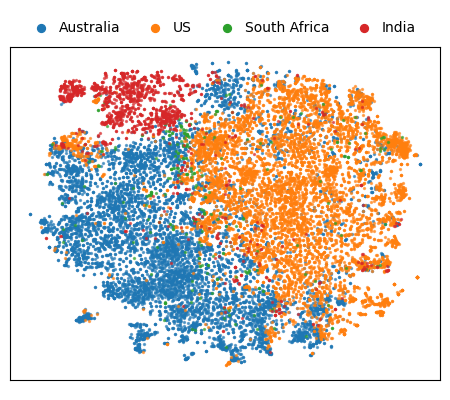
\includegraphics[width=1\linewidth]{img/tsne_ncountry.png}
\caption{T-SNE projection from 768 dimensional representation of Bert's last hidden layer (averaged). Each dot represents one article the body of which has been embedded (first 512 subwords). Axes hidden intentionally.}
\label{fig:tsne}
\end{figure}

\subsection{Evaluation} \label{subsec:evaluation}

Because there is no single task that we are trying to solve, we do not have a single form of the dataset on which to run all the experiments.
To answer some research questions, we craft new datasets by combining some of the answers as cues in the input.
Unless stated otherwise, we use 1k articles for the development set and 1k articles for the test set (both randomly sampled articles for development).
The filtered and preprocessed dataset is described in \Cref{subsec:data}.

We combine two metrics for task evaluation.
For variables with unique outputs (\emph{month, year, newspaper, news. alignment and news. country}) we use accuracy.\footnote{
Despite the class imbalance, we report the results in accuracy for clarity and ease of comparison because we are not interested in the absolute task performances but rather in the differences between models.
Albeit sometimes misleading, accuracy is very intuitive and easy to interpret and the output is always a single number, which we need because of the large number of evaluations.
}
For variables that are a non-empty subset of the output domain (\emph{subject, geographical}) we assume that the model is able to order the items (commonly used scoring).
We utilize that to compute R-Precision from the output against the correct classes.
Given the correct non-empty set of items $Y$, we take $|Y|$ top-scoring (by probability) items from the predictions and compute the overlap:
$$
RPrec(Y, \hat{Y}) \defeq \frac{|(\arg \max_{|Y|}\hat{Y}) \cap Y|}{|Y|}
$$

This is a common metric for information retrieval \cite{Beitzel2009} which can also be used for our purposes.
The alternative would be either to (1) compute average item accuracy which would almost always force models to predict the item not present due to data sparsity or (2) merge the items into balanced clusters.
Even though the latter option is viable, we chose to use R-Precision not to have all tasks in the multi-task settings use the same evaluation scheme.

\section{Experiments} \label{sec:experiments}

We first document the pairwise variable dependency and then build single and joint models for their prediction.
We follow up by fusing the variables as artefacts to the main model and studying its effects.
Finally, we build a meta-model used for automatically determining the need for the provision of artefacts to the main model.

\subsection{Variable Dependency} \label{subsec:feature_dependency}

Naturally, some features are fully interdependent.
For example, \emph{newspaper alignment} is fully determined by \emph{newspaper} (although not vice versa).
It would be possible to depict this dependency using the $\chi^2$ statistics, though it would become problematic with features that are subsets (\emph{subject}, \emph{geographic}).
One solution would be to exponentially expand this into unique classes which we avoided because of the unreasonably large output space $({>}2^{81})$.
Instead, we treat one variable as the sole input to the model while another variable as the output.
This allows us to make comparisons with later, more informed models.
For the model, we use unregularized multinomial logistic regression (each output label is predicted independently).\footnote{
This model was chosen for its simplicity and also its similarity to the computation of the Bert-based model head: linear projection with a softmax.
}
Formally this would correspond to predicting $z\in y$ such that:
$\hat{z} = p(-,\xi;\, \theta),\,\, \xi \in y$.

We measure these results using training accuracy because we are interested in the possible limits of information that can be extracted between the classes.
For \emph{subject} and \emph{geographic} we train individual logistic regressions for every item and use the output probabilities for predicting the item being present as scores.
The results are presented in \Cref{fig:feature_dependency_lr}.
Baseline (random) results are presented in the topmost row.
For accuracy-based variables, we used the most common class classifier while for R-Precision based ones, we used the feature frequency as the scoring vector for metric computation.
Formally this random classifier predicts: $z\in y$ such that $\hat{z} = p(-,-;\theta)$.

\begin{figure}[ht]
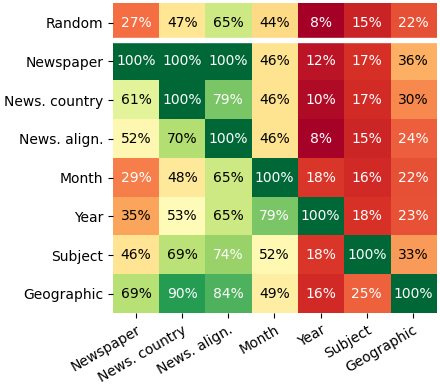
\includegraphics[width=1\linewidth]{img/feature_dependency_lr.png}
\caption{Logistic regression between input variable (row) to predicted variable (column). Performance is reported in training accuracy except for variables \emph{subject} and \emph{geographic} which are reported with R-Precision.}
\label{fig:feature_dependency_lr}
\end{figure}

Naturally, everything is better than the random model though not all variable directions by a large margin.
The dependency of newspaper attributes on \emph{newspaper} is demonstrated by the 100\% accuracy.
This is also naturally true for the features predicting themselves.
We can also see that there is some relationship between the \emph{subject} and \emph{geographic} variables.
\emph{Newspaper} also predicts the \emph{geographic} variable better than randomly.
Note that it is not rational to expect the same improvements over baseline for the main model because of non-zero joint information of $x$ and $\xi$.

\subsection{Models Without Artefacts}

\subsubsection{Bert-Single}
The input to the Bert model is the first 512 subword units of the body.
Even though this may not be the most informative part of the article and better heuristics exist, we keep this to be consistent across all configurations.
The results are presented in the left column of \Cref{tab:bert_single_multi}.
In comparison to the baselines, the model seems to be only slightly better.
The Bert model however has access to much less data than the baseline models (on average, articles have almost 1k words).
One possible solution to this would be to combine the TF-IDF vector with the Bert representation, as done for LSTM, and use it jointly for classification head input.
The Bert model seems to have a strong advantage for the \emph{subject} and \emph{geographic} variables.

\begin{table}[ht]
\centering
\begin{tabular}{lccc}
\toprule
& Bert-Single & Bert-Joint \\
\midrule
Newspaper & \prc{86.8}  & \prc{86.4} \\
News. country & \prc{98.3} & \prc{98.4} \\
News. align. & \prc{92.7} & \prc{94.8} \\
Month & \prc{59.8} & \prc{53.5} \\
Year & \prc{43.0} & \prc{18.0} \\ 
\midrule
% r-precision
Subject & \prc{75.8} & \prc{54.1} \\
Geographic & \prc{81.2} & \prc{46.3} \\
\bottomrule
\end{tabular}
\caption{
Comparison of individual and multi-output prediction using Bert.
Performance is reported in development accuracy except for variables \emph{subject} and \emph{geographic} which are reported with R-Precision. The joint Bert model is trained using uniform loss averaging.
}
\label{tab:bert_single_multi}
\end{table}

\subsubsection{Bert-Joint}
We now turn our focus on the different ways we explored to train a joint classification model.
Specifically, we look at how the loss reduction criteria affects the level of optimization of each variable.
We consider three loss reduction approaches, uniform loss averaging, weighted loss averaging (scaling down the loss of multi-output targets) and root squared mean (RSM, power mean $n=2$) averaging.
The comparison of Bert-Joint (Uniform) to Bert-Single is presented in \Cref{tab:bert_single_multi}.
The performance is comparable on newspaper-related variables and worse on the rest.
The results for different loss reduction methods are shown in \Cref{tab:bert_multi}.

\begin{table}[ht]
\centering
\begin{tabular}{lccc}
\toprule
& Uniform & Weighted & RSM \\
\midrule
Newspaper & \prc{86.4} & \prc{87.1} & \prc{86.4}\\
News. country\hspace{-0.2cm} & \prc{98.4} & \prc{98.4} & \prc{98.7}\\
News. align. & \prc{94.8} & \prc{94.6} & \prc{94.7} \\
Month & \prc{53.5} & \prc{57.9} & \prc{61.0}\\
Year & \prc{18.0} & \prc{37.1} & \prc{41.5}\\ 
\midrule
% r-precision
Subject & \prc{54.1} & \prc{25.1} & \prc{33.7}\\
Geographic & \prc{46.3} & \prc{35.4} & \prc{25.6}\\
\bottomrule
\end{tabular}
\caption{
Comparison of different loss reduction criteria for the Bert-Joint model and their effect on the optimization of the classified variables.
}
\label{tab:bert_multi}
\end{table}

All the three modes for loss aggregation perform similarly in variables \emph{newspaper}, \emph{newspaper country} and \emph{newspaper alignment}.
There is, however, a large difference in performance in the other targets, especially for the variable \emph{year} and the multi-output targets (\emph{subject} and \emph{geographic}).
Although no method dominates the rest, we conclude that the uniform method is more attractive if we leave out the \emph{year} variable and, if desirable, train a single model just for this difficult variable.

\subsection{Provision of Artefacts}

\subsubsection{Single Artefact}

We start the fusion exploration by providing only one other variable, which is comparable to \Cref{subsec:feature_dependency}.
We prepend the specific variable to the model input.
For \emph{subject} and \emph{geographic} we select only two of the shortest items (for each article) to use as an artefact.
This is motivated by the limited Bert input capacity as well as empirical results for the best performance.

The results, shown in \Cref{fig:feature_dependency_bert} show similar patterns to that of just using the artefact for prediction.
In multiple cases, the performance dropped which may be caused by one of the potential issues described in \Cref{subsec:related}, such as taking up input space and more complex optimization algorithm.
Strangely the performance for the \emph{year} variable decreased greatly when using \emph{geographic} as an artefact.
% We looked for bugs but found none and we ultimately could not find a reasonable explanation for this behaviour.
For this phenomenon, we are currently unable to provide any explanation.
% The \emph{year} variable behaves very strangely throughout all results and would require further study.

\begin{figure}[ht]
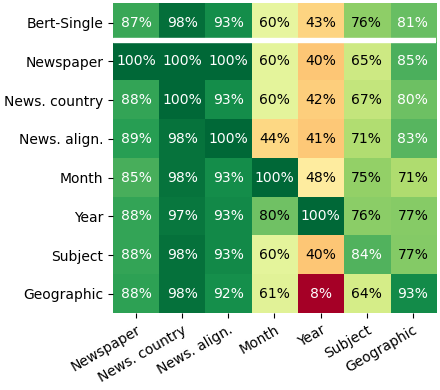
\includegraphics[width=1\linewidth]{img/bert_1v1_heatmap.png}
\caption{Performance of predicting the variable in column using Bert model when the input variable (row) is prepended to the input. Performance is reported in training accuracy except for variables \emph{subject} and \emph{geographic} which are reported with R-Precision.}
\label{fig:feature_dependency_bert}
\end{figure}

\subsubsection{Multiple Artefacts} \label{subsubsec:multiple_artefacts}

We consider two levels in which to mediate access to the multiple artefacts.
In the first one, all other variables are stringified together and prepended to the input (headline).
This corresponds to predicting $z \in y$ such that $\hat{z} = p(x, \xi;\theta), \xi = y \mysetminus z$.
We do not include \emph{newspaper country} and \emph{newspaper alignment} in $\xi$ because they can be uniquely inferred from \emph{newspaper}.
In the second, we randomly drop out the information by with 50\% chance.
Note that this is not the same as dropout for neural networks, because the dropout filter for one specific sample is generated in every batch.
In our case, the dropout is applied on the level of data and stays fixed for the whole of training.
We mask the dropped out items with the token \texttt{None}.\footnote{Other options would be to use a different token or to skip it altogether. The token \texttt{None} worked sufficiently well enough to not warrant further search.}

For evaluation presented in \Cref{tab:multi_dropout}, we use the unmodified data as well as dropout levels 50\% and 100\%.
These results help us see systematic (and gradual) improvement when artefacts are provided.
It also demonstrates that even when the artefacts are provided only sometimes, the model is able to make use of them, making it more versatile regarding the input.

\begin{table}[ht]
\centering
\begin{tabular}{lccc}
\toprule
% 25% artefacts corresponds to 75% dropout on our side
Artefacts & 100\% & 50\% & 0\% \\
\midrule
Newspaper & \prc{88.5} & \prc{87.9} & \prc{86.8} \\
News. country & \prc{100\,} & \prc{98.9} & \prc{98.3} \\
News. align. & \prc{100\,} & \prc{96.7} & \prc{92.7}\\
Month & \prc{80.3} & \prc{69.7} & \prc{54.3}\\
Year & \prc{52.2} & \prc{43.7} & \prc{43.0}\\ 
\midrule
% r-precision
Subject & \prc{75.0} & \prc{75.9} & \prc{75.8}\\
Geographic & \prc{85.5} & \prc{82.0} & \prc{81.2}\\
\bottomrule
\end{tabular}
\caption{
Individual Bert performances were measured by accuracy and R-Precision when fused with extra artefacts (all other output variables).
Percentages in columns indicate the percentage that is preserved after a fixed single pass of dropout.
}
\label{tab:multi_dropout}
\end{table}

\subsubsection{Predicting Need for Help} \label{subsubsec:need_help}

The 50\% dropout model with multiple artefacts from \Cref{subsubsec:multiple_artefacts} demonstrated that it is possible to have a single model that works both with and without artefacts.
Based on the model for predicting \emph{month} variable,\footnote{We choose this variable not because of any applicable interest but because of the large difference in performance when artefacts are supplied.} we construct the following dataset.
The class is \texttt{1} if the model predicted the output correctly and \texttt{0} otherwise.
The input is either the last hidden state of Bert for the \texttt{[CLS]} token or the softmax output (posterior).
This is joined by a binary vector indicating which artefacts were used.
For the trained model we add the individual artefacts and store the output correctness.
The target output of this task is a variable that determines whether the classification is likely to be correct.
This is illustrated in \Cref{fig:meta_model}.

\begin{figure}[ht]
\centering
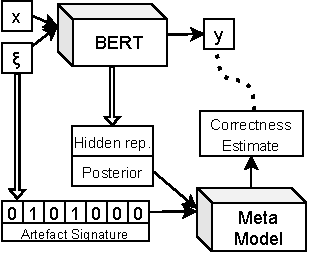
\includegraphics[width=0.85\linewidth]{img/meta_model.pdf}
\caption{Pipeline of estimating correctness of model output using a meta-model (either \emph{true posterior} or \emph{frozen posterior}).}
\label{fig:meta_model}
\end{figure}

To apply this model, we may start by providing no artefacts and finish if the prediction is that the output will be correct (or when the confidence of the meta-model is high enough).
If not, then we may add an artefact to the model and evaluate the meta-model again.
We denote this model as \emph{true posterior}.
This approach requires access to the given artefact in order to evaluate the success chance.
It is however possible to simply change the artefact signature and keep the posterior from the computation without any artefacts.
This has the advantage of practically being able to determine which artefact increases the chance of correctness the most.
We refer to this model as \emph{frozen posterior}.
Lastly, it is possible to not use the artefact signature as an input but make the model output estimates whether the computation with added $i$-th artefact results in a correct output.
We refer to this as \emph{joint $\xi$ estimate}.
Although it is possible to use this model to predict success without an artefact, the model is not able to predict the success chance with more than one artefact added.
A possible solution would be to consider a subset of artefacts as atomics which however leads to exponentially large output vectors.

The output classes for success are either \emph{positive} or \emph{negative} and we, therefore, evaluate the models for a binary classification task and report precision (motivated by data imbalance).\footnote{
We report precision instead of $F_1$ score because it reveals more insight in comparison to the most common class classifier which trivially achieves 100\% recall.
}
We consider only four artefacts for the base model that predicts the \emph{month} variable: \emph{newspaper}, \emph{newspaper alignment}, \emph{newspaper country} and \emph{year}.

The first two models are a simple feed-forward neural network with the input of posterior (softmaxed), artefact signature and the last-layer representation for the \texttt{[CLS]} token.
The 768-dimensional representation from Bert is dropped out with 75\% probability while the posterior and the signature are left intact.
This is followed up by two hidden layers with 64 nodes and ReLU activations.
The networks are optimized with Adam \cite{kingma2017adam}, learning rate 10$^{-3}$, within batches of 128 and cross-entropy loss (two output nodes for positive and negative predictions).
The last model, \emph{joint $\xi$ estimate}, follows this architecture with the last layer containing (4+1)$\times$2 nodes.
The loss is applied to each pair which corresponds to positive and negative predictions for each of the individual artefacts and also case without any artefacts.

The results are presented in \Cref{tab:meta_model}.
In the first column, we measure how well the meta-models are able to determine success without an artefact.
In the second column, the base model was fused with exactly one input artefact and in the last column with an arbitrary non-empty subset of them.
Note that for the train/dev evaluation split, we split at sample boundaries to prevent unwanted leakage of information from training data to development.
The first two models were trained separately for each column while the last model was trained only once.
We list the most common class classifier (positive) as the baseline for comparison.

\begin{table}[ht]
\centering
\begin{tabular}{lccc}
\toprule
Model & No $\xi$ & Indiv. $\xi$ & Mult. $\xi$ \\
\midrule
MCCC & \prc{64.5} & \prc{65.7} & \prc{69.0} \\
True posterior &
\prc{75.0} & \prc{92.0} & \prc{80.7} \\
Frozen posterior \hspace{-0.4cm} &
\prc{75.0} & \prc{78.5} &\prc{79.4} \\
Joint $\xi$ estimate &
\prc{80.0} & \prc{79.5} & -  \\
\bottomrule
\end{tabular}
\caption{Precisions of meta models for predicting classification success. Bottommost row shows the averaged base model accuracy on the \emph{month} classification task.}
\label{tab:meta_model}
\end{table}

Even though the results are not perfect, it is clear that there is information stored in the posteriors and the hidden representation that allows the meta-models to determine the success better than random.
As expected, the meta-model with frozen posterior is systematically worse than with access to the true posteriors (and hidden representation).
Interestingly, predicting the probabilities for each artefact (and no artefact) jointly is not only more effective but also outperforms the other two models which take the artefact signature as an input.

\subsection{Tracing Fusion Effect}

We examine how the fusion of the artefacts affects the model computation.
For that purpose, we show distances on the between (1) computation which was not provided with artefacts and (2) one which used at least one artefact:
$$
L^2[o_i(x,-;\theta), o_i(x,\xi;\theta)], \xi \neq \emptyset
$$
We distinguish between cases based on the correctness of the original prediction and on whether the fusion helped or worsened the enhanced prediction.
The model, same as for \Cref{subsubsec:need_help}, predicts the \emph{month} variable and is trained with static 50\% artefact dropout.
Similar to \newcite{zouhar2021artefact}, we view the model computation as a composition of functions that each creates an intermediate projection.
We limit ourselves by considering the hidden state representation only for the \texttt{[CLS]} token\footnote{The choice of considering the representation for the \texttt{[CLS]} token for deeper layers was arbitrary and we treat it as a representation (for the computation related to the classification) of the whole layer.} on the $i$-th layer but include also the classification layer, its softmax and the one-hot encoded prediction.

\begin{figure}[ht]
\centering
\vspace{0.5cm}
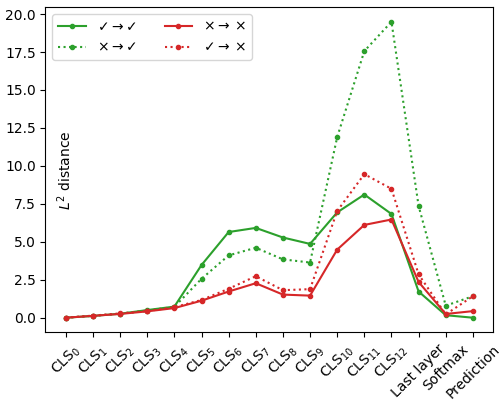
\includegraphics[width=1\linewidth]{img/fusion_tracing.png}
\caption{Distances of projections (either \texttt{[CLS]} token or whole layers) between no fusion and fusion of at least of artefact.}
\label{fig:fusion_tracing}
\end{figure}

The distances, for all available data, are shown in \Cref{fig:fusion_tracing}.
There is a clear distinction between the different cases with the artefact making the prediction correct ($\times \rightarrow \checkmark$) being the most distinct (largest divergence from no fusion).
Interestingly enough, the computations diverge only from the fifth layer and not before.
This is in contrast to the intuition that the signal from early fusion gets lost and disregarded later in the computation.
The fact that the distances between predictions for $\times \rightarrow \times$ are neither 0 nor $\sqrt{2}$ means that the fusion of the artefact changed some of the wrong predictions but not to the correct ones.

Note that the vector spaces at every layer are different and therefore also the metrics defined on these spaces are scaled differently.
For example dimension-averaged variance of $\text{CLS}_{12}$ is greater than the dimension-averaged variance of $\text{CLS}_{2}$.
It is however still possible to compare the proportions of distances between the different configurations, which yield the same results.

\section{Conclusion} \label{sec:conclusion}

% Q1:
We examined a specific case of multi-task classification, which we found to be slightly outperformed by the individual models in some cases but with the benefit of increased efficiency.
% Q2:
We then used the output variables for fusion as artefacts and showed that they can systematically improve the predictions.
% Q3:
We built a meta-model that predicted whether the base model will be correct or not and if an infusion of certain artefact(s) will help.
Even though this meta-model provided only a baseline, it showed that it is possible to predict the need for artefacts.
% Q4:
Lastly, we explored the artefact fusion from the perspective of diverging computation trajectories and saw clear distinctions between cases in which the original prediction was correct or not and whether the artefact helped or worsened the prediction.

\paragraph{Future work.}

We identify the following areas for future research:

\begin{itemize}[left=0.0cm,topsep=0.1cm,noitemsep]
\item Exploring loss reduction criteria more in-depth to allow better performance with joint classification models.
\item Examining model confidence when artefacts are provided or on samples from unseen classes.
\item Replicating the experiments for other fusion methods apart from priming, such as adding vectors to the intermediate computation or constraining the output.
\item Exploring artefact dependency and the need for its provision could be examined also by the attention mechanism in pre-trained language models that utilize it.
\item Provision of misleading artefacts (adversarial conditions) and model robustness.
\end{itemize}

\paragraph{Division of work.}

While Vilém designed the experiments, paper, presentation and managed data generation, meta models and baselines, Edu prepared, trained and evaluated the Bert models and documented the corresponding parts.